% Type of the document
\documentclass{beamer}

% elementary packages:
\usepackage{graphicx}
\usepackage[latin1]{inputenc}
\usepackage[T1]{fontenc}
\usepackage[english]{babel}
\usepackage{listings}
\usepackage{xcolor}
\usepackage{eso-pic}
\usepackage{mathrsfs}
\usepackage{url}
\usepackage{amssymb}
\usepackage{amsmath}
\usepackage{multirow}
\usepackage{hyperref}
\usepackage{booktabs}
\usepackage{tikz}

% additional packages
\usepackage{bbm}

% packages supplied with ise-beamer:
\usepackage{cooltooltips}
\usepackage{colordef}
\usepackage{beamerdefs}
\usepackage{lvblisting}

% Change the pictures here:
% logobig and logosmall are the internal names for the pictures: do not modify them. 
% Pictures must be supplied as JPEG, PNG or, to be preferred, PDF
\pgfdeclareimage[height=2cm]{logobig}{hulogo}
% Supply the correct logo for your class and change the file name to "logo". The logo will appear in the lower
% right corner:
\pgfdeclareimage[height=0.7cm]{logosmall}{Figures/hulogo}

% Title page outline:
% use this number to modify the scaling of the headline on title page
\renewcommand{\titlescale}{1.0}
% the title page has two columns, the following two values determine the percentage each one should get
\renewcommand{\titlescale}{1.0}
\renewcommand{\leftcol}{0.6}

% Define the title.Don't forget to insert an abbreviation instead 
% of "title for footer". It will appear in the lower left corner:
\title[Predicting House Prices using Machine Learning]{The title of the talk can even be much longer than this}
% Define the authors:
\authora{Dennis Koehn} % a-c
\authorb{Linxi Wang}
\authorc{Mingyang Li}

% Define any internet addresses, if you want to display them on the title page:
\def\linka{http://lvb.wiwi.hu-berlin.de}
\def\linkb{www.case.hu-berlin.de}
\def\linkc{}
% Define the institute:
\institute{Ladislaus von Bortkiewicz Chair of Statistics \\
C.A.S.E. -- Center for Applied Statistics\\
    and Economics\\
Humboldt--Universit{\"a}t zu Berlin \\}

% Comment the following command, if you don't want, that the pdf file starts in full screen mode:
\hypersetup{pdfpagemode=FullScreen}

%%%%
% Main document
%%%%
\begin{document}
% Draw title page
\frame[plain]{%
\titlepage{}
}

% The titles of the different sections of you talk, can be included via the \section command. The title will be displayed in the upper left corner. To indicate a new section, repeat the \section command with, of course, another section title
%%%%%%%%%%%%%%%%%%%%%%%%%%%%%%%%%%%%%%%%%%%%%%%%%%%%%%%%%%%%%%%%%%%%%%%%%%%%%%%%%%%%%%%%%%%%%%%%%%%%%%%%%%%%%%%%%%%%%%%%
%%%%%%%%%%%%%%%%%%%%%%%%%%%%%%%%%%%%%%%%%%%%%%%%%%%%%%%%%%%%%%%%%%%%%%%%%%%%%%%%%%%%%%%%%%%%%%%%%%%%%%%%%%%%%%%%%%%%%%%%
\frame{
\frametitle{Outline}

\begin{enumerate}
\item Introduction \quad \checkmark
\item Pre-processing Steps
\item Model Selection
\item Variable Importance and Dimensionality Reduction 
\item Results
\item Conclusion and Outlook
\end{enumerate}
}

\section{Introduction}
%%%%%%%%%%%%%%%%%%%%%%%%%%%%%%%%%%%%%%%%%%%%%%%%%%%%%%%%%%%%%%%%%%%%%%%%%%%%%%%%%%%%%%%%%%%%%%%%%%%%%%%%%%%%%%%%%%%%%%%%

% (A numbering of the slides can be useful for corrections, especially if you are
% dealing with large tex-files)
%%%%%%%%%%%%%%%%%%%%%%%%%%%%%%%%%%%%%%%%%%%%%%%%%%%%%%%%%%%%%%%%%%%%%%%%%%%%%%%%%%%%%%%%%%%%%%%%%%%%%%%%%%%%%%%%%%%%%%%%
\frame{
\frametitle{Formal Problem Setting}
\begin{itemize}
\item \textit{training set}: inputs $X = (x_1,\dots,x_n) \in \mathbb{R}^{n \times d}$ and labels $Y = (y_1,\dots,y_n)  \in  \mathbb{R}^{n}$
\item  \textit{test set}: inputs $X' = (x'_1,\dots,x'_t) \in \mathbb{R}^{t \times d}$ without labels
\end{itemize}
\vspace{0.5cm}
Find a function 
\begin{align}
f: X\rightarrow Y 
\end{align}
s.t. the labels of \textit{test set} are predicted as accurately as possible, i.e.
\begin{align}
f(X') \approx Y'
\end{align} 
}

\frame{
\frametitle{Ames House Price Data}
\vspace{0.25cm}
Characteristics and Sale Price of Houses in Ames, Iowa provided by \href{https://www.kaggle.com/}{kaggle.com}:
\begin{itemize}
\item 79 variables as inputs plus sale price in the training set
\item 1460 Observations in training set
\item 1459 Observations in test set (thus 1459 labels to predict) 
\end{itemize}
\vspace{0.5cm}
Only Kaggle knows the 1459 Labels of the test set. We submitted our predictions at the website and obtain the RMSE of the log labels.
\begin{align*}
RMSE = \sqrt{\dfrac{1}{t} \sum_{i=1}^{t} \Big( log(\hat{y}_i) - log(y'_i) \Big)^2}
\end{align*}

}

\section{Pre-Processing}
 
\frame{
\vspace{0.1cm}
Several transformations and cleaning steps needed before putting the data into an algorithm, e.g. 
\frametitle{Pre-processing}

\begin{figure}
	\begin{center}
	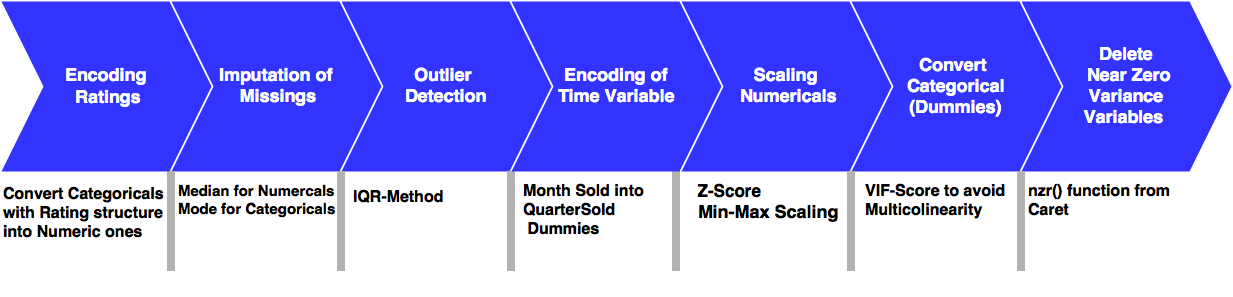
\includegraphics[scale=0.25]{Figures/DataPipeline-1.jpg}
	\caption{Workflow of Pre-Processing Steps}
	\label{fig:DataPipeline}
	\end{center}
\end{figure}
All transformation need to be preformed on the test set as well! 
}

\begin{frame}[fragile]
\begin{center}
\begin{lstlisting}
basic_preprocessing = function(X_com, y, scaler="gaussian") 
{
	source("replace_ratings.R")
	source("convert_categoricals.R")
	source("impute_data.R")
	source("encode_time_variables.R")
	source("impute_outliers.R")
	source("scale_data.R")
	source("delete_nearzero_variables.R")
    X_ratings = replace_ratings(X_com)
    X_imputed = naive_imputation(X_ratings)
    X_no_outlier = data.frame(lapply(X_imputed, iqr_outlier))
    X_time_encoded = include_quarter_dummies(X_no_outlier)
\end{lstlisting}
\end{center}
\quantnet \href{https://github.com/koehnden/SPL16/tree/master/Quantnet/dataProcessing/}{dataProcessing}
\end{frame}

\begin{frame}[fragile]
\begin{center}
\begin{lstlisting}
 	X_scaled = scale_data(X_time_encoded, scale_method = scaler)
    X_encoded = data.frame(lapply(X_scaled, cat_to_dummy))
    X_com = delect_nz_variable(X_encoded)
    idx_train = c(1:length(y))
    train = cbind(X_com[idx_train, ], y)
    test = X_com[-idx_train, ]
    return(list(train = train, X_com = X_com, test = test))
}
\end{lstlisting}
\end{center}
\quantnet \href{https://github.com/koehnden/SPL16/tree/master/Quantnet/dataProcessing/}{dataProcessing}
\end{frame}

 

\section{Model Selection}

\begin{frame}
\frametitle{Considered Algorithms}
\begin{itemize}
\item Random Forest from \texttt{library('h2o')}
\begin{itemize}
\item tuning \texttt{max\char`depth},  \texttt{gamma} and \texttt{sample\char`_size}
\item determining \texttt{ntree} through \texttt{early\char`_stopping()} option
\end{itemize}
\item Gradient Boosting Machines from \texttt{library('xgboost')}
\begin{itemize}
\item tuning  \texttt{max\char`_depth}, \texttt{gamma} \texttt{subsample} and \texttt{col\char`_by\char`_tree}
\item determining \texttt{nrounds} through \texttt{early\char`_stopping()} option
\end{itemize}
\item Support Vector Regression with Gaussian Kernel from \texttt{library('kernlab')} 
\begin{itemize}
\item tuning \texttt{lambda} and \texttt{sigma} via \texttt{caret} 
\end{itemize}
\end{itemize}	
\end{frame}

%%%%%%%%%%%%%%%%%%%%%%%%%%%%%%%%%%%%%%%%%%%%%%%%%%%%%%%%%%%%%%%%%%%%%%%%%%%%%%%%%%%%%%%%%%%%%%%%
\begin{frame}[fragile]
\frametitle{Optimizing Hyper-parameters} 

\begin{figure}
	\begin{center}
	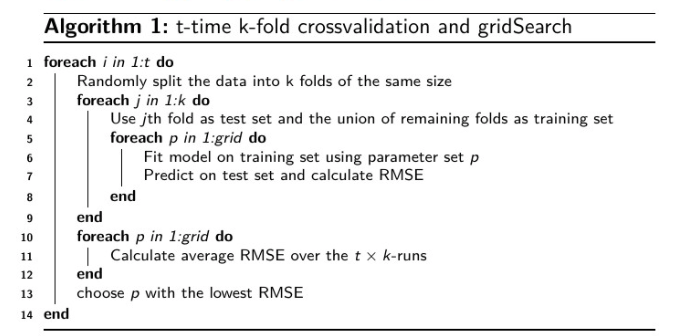
\includegraphics[scale=0.43]{Figures/OHP.jpg}
%	\caption{Workflow of Pre-Processing Steps}
%	\label{fig:DataPipeline}
	\end{center}
\end{figure}


\quantnet \href{https://github.com/koehnden/SPL16/tree/master/Quantnet/xgbTuning/}{xgbTuning}
\quantnet \href{https://github.com/koehnden/SPL16/tree/master/Quantnet/rfTuning/}{rfTuning}
\quantnet \href{https://github.com/koehnden/SPL16/tree/master/Quantnet/svmTuning}{svmTuning}
\end{frame}


%%%%%%%%%%%%%%%%%%%%%%%%%%%%%%%%%%%%%%%%%%%%%%%%%%%%%%%%%%%%%%%%%%%%%%%%%%%%%%%%%%%%%%%%%%%%%%%%
\frame{
\frametitle{GBM tunning results}
\begin{figure}
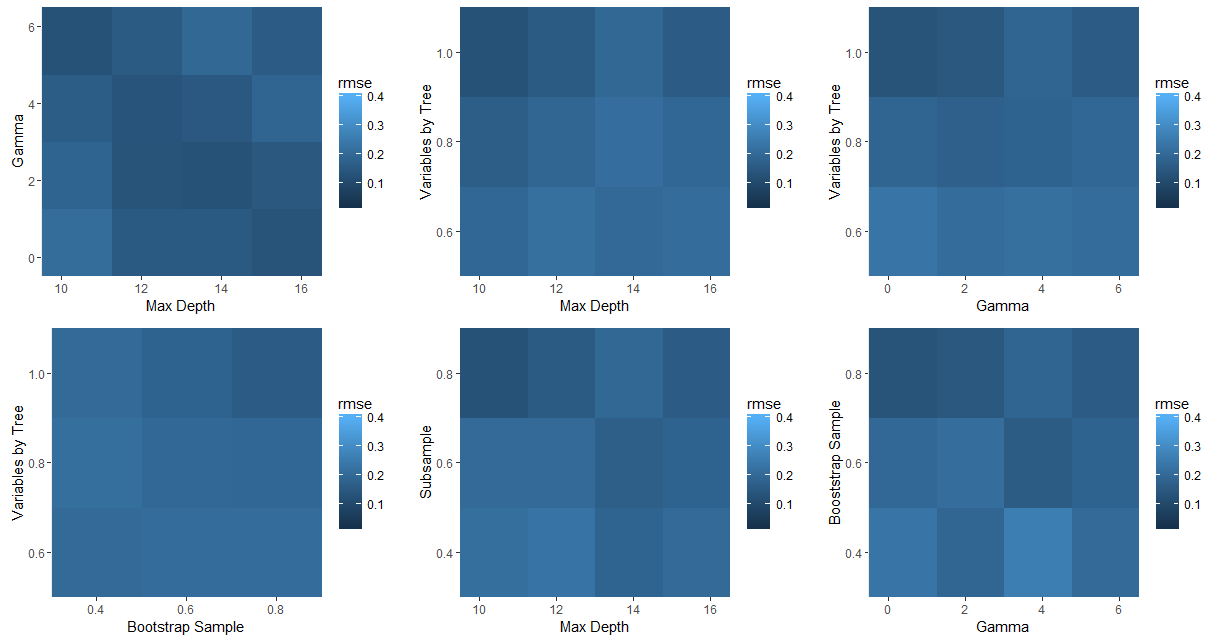
\includegraphics[scale = 0.26]{figures/tuning_heatmap_xgb.jpg} 
\caption{Heatmap of GBM tuning results}
\end{figure}
\quantnet \href{https://github.com/koehnden/SPL16/tree/master/Quantnet/xgbTuning/}{xgbTuning}
}

\section{Variable Importance and Dimensionality Reduction}

%%%%%%%%%%%%%%%%%%%%%%%%%%%%%%%%%%%%%%%%%%%%%%%%%%%%%%%%%%%%%%%%%%%%%%%%%%%%%%%%%%%%%%%%%%%%%%%%
\frame{
\frametitle{Taking on the curse of dimensionality}
Problem: 
\begin{itemize}
\item many variable (99 after pre-processing)
\item small training set ($n = 1460$) 
\item variables are correlated with each other
\end{itemize}
\vspace{0.1cm}
Our approaches:
\begin{itemize}
\item Variable selection through variable importance ranking
\item Extract a smaller set of variable using PCA
\end{itemize}
}


%%%%%%%%%%%%%%%%%%%%%%%%%%%%%%%%%%%%%%%%%%%%%%%%%%%%%%%%%%%%%%%%%%%%%%%%%%%%%%%%%%%%%%%%%%%%%%%% 
%TODO: Change Slide into two slides with bigger plot
\frame{
\frametitle{Variable Importance of Tree-Based Methods}
\begin{figure}
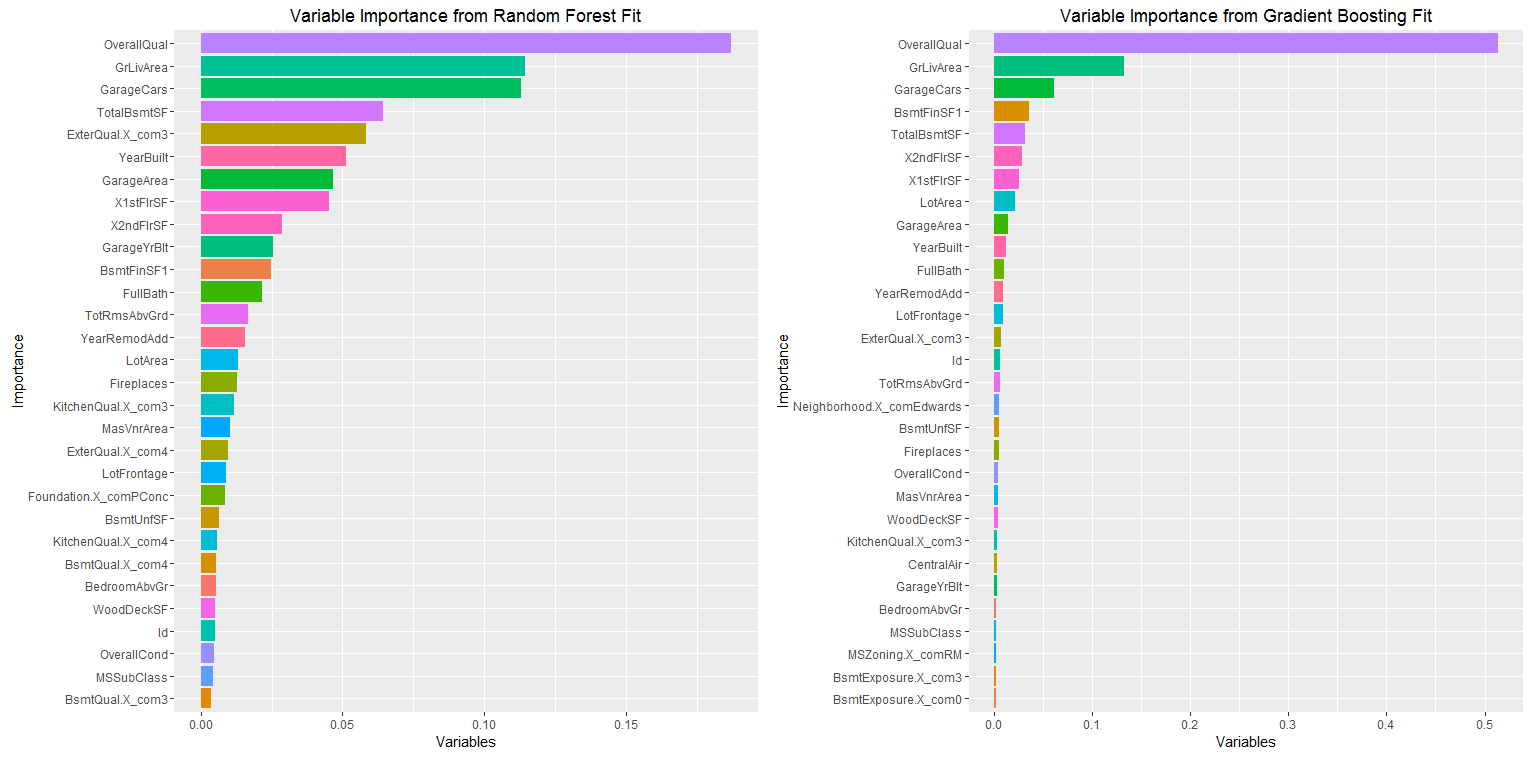
\includegraphics[scale = 0.22]{figures/top_30_varimp_xgb_rf.jpg} 
\caption{RF vs. GBM Variable Importance}
\end{figure}
\quantnet \href{https://github.com/koehnden/SPL16/tree/master/Quantnet/rfFeatureSelection/}{rfFeatureSelection}
\quantnet \href{https://github.com/koehnden/SPL16/tree/master/Quantnet/xgbFeatureSelection/}{xgbFeatureSelection}
}


%%%%%%%%%%%%%%%%%%%%%%%%%%%%%%%%%%%%%%%%%%%%%%%%%%%%%%%%%%%%%%%%%%%%%%%%%%%%%%%%%%%%%%%%%%%%%%%%
\frame{
\frametitle{Recursive Feature Elimination using SVR}
\begin{itemize}
	\item Recursive Feature Elimination suggests that the full set of variables performs best
\end{itemize}
\begin{figure}
% TODO different shape of the plot
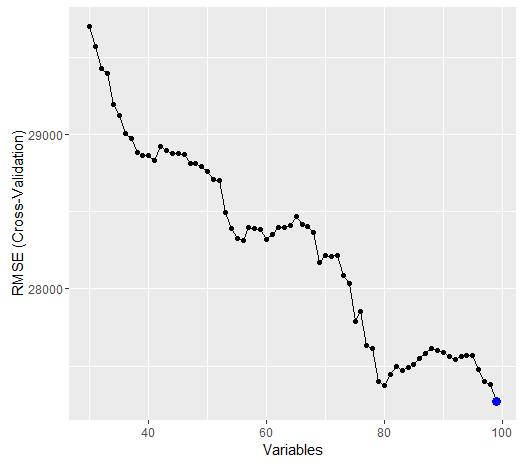
\includegraphics[scale = 0.26]{figures/svmRFEplot.jpg} 
\caption{RFE using SVR with Gaussian Kernel}
\label{fig:RFE}
\end{figure}
\quantnet \href{https://github.com/koehnden/SPL16/tree/master/Quantnet/svmRFE}{svmRFE}
}


%%%%%%%%%%%%%%%%%%%%%%%%%%%%%%%%%%%%%%%%%%%%%%%%%%%%%%%%%%%%%%%%%%%%%%%%%%%%%%%%%%%%%%%%%%%%%%%%
\frame{
\frametitle{Principal Component Analysis}
\begin{itemize}
	\item We use the first 55 principal components as input data, which make up 0.8 of the total variance
\end{itemize}
\begin{figure}
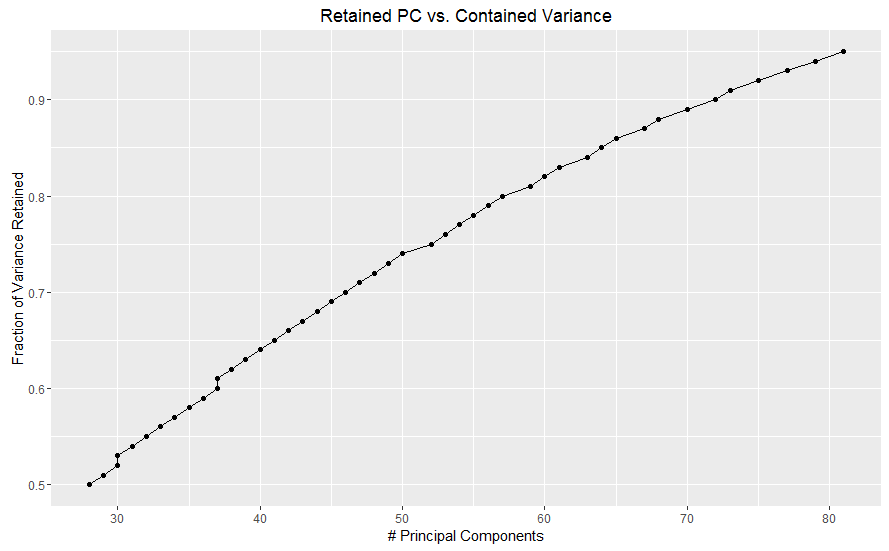
\includegraphics[scale = 0.22]{figures/reverse_elbow_plot.jpg} 
\caption{Reverse Elbow Plot}
\end{figure} 
\quantnet \href{https://github.com/koehnden/SPL16/tree/master/PCA/}{PCA}
}

\section{Final Models}


%%%%%%%%%%%%%%%%%%%%%%%%%%%%%%%%%%%%%%%%%%%%%%%%%%%%%%%%%%%%%%%%%%%%%%%%%%%%%%%%%%%%%%%%%%%%%%%%
\frame{
\frametitle{Results}
\begin{itemize}
\item Gaussian SVR with all variable is the single best model
\item PCA did not work well 
\item Models perform best with the full set of variables as Figure \ref{fig:RFE} suggested 
\end{itemize}
\vspace{0.25cm}
\begin{table}
\begin{center}
\begin{tabular}{c|ccc} 
\hline\hline
Inputs 		  & Gaussian SVR    & Random Forest & GBM      \\ 
\hline 
All Variables & \textbf{0.1308} &  0.1484       & 0.1333   \\
Top 30 		  & 0.1323  	 	&  0.1515       & 0.1436    \\
PCA	   		  & 0.1607  	    &  0.1657       & 0.1657     \\
\hline\hline
\end{tabular}
\caption{RMSE of submitted predictions}
\end{center}
\end{table}
\quantnet \href{https://github.com/koehnden/SPL16/blob/master/finalModels.R}{finalModels}
}


%%%%%%%%%%%%%%%%%%%%%%%%%%%%%%%%%%%%%%%%%%%%%%%%%%%%%%%%%%%%%%%%%%%%%%%%%%%%%%%%%%%%%%%%%%%%%%%%
\frame{
\frametitle{Conclusion and Outlook}
\begin{itemize}
\item Unexpected result: SVR outperforms the tree-based ensembles
\begin{itemize}
\item SVR benefits more from pre-processing steps e.g. outlier detection and scaling 
\end{itemize}

\item further improvement possible by
\begin{itemize}
\item building ensembles different models
\item detailed feature engineering
\end{itemize}
\end{itemize}

}


%%%%%%%%%%%%%%%%%%%%%%%%%%%%%%%%%%%%%%%%%%%%%%%%%%%%%%%%%%%%%%%%%%%%%%%%%%%%%%%%%%%%%%%%%%%%%%%%
% Dedicated section for references
\frame{
\frametitle{References}
\begin{thebibliography}{aaaaaaaaaaaaaaaaa}
\beamertemplatearticlebibitems
\bibitem{Blei, David M., Andrew Y. Ng, and Michael I. Jordan:2003}
Blei, David M., Andrew Y. Ng, and Michael I. Jordan
\newblock{\em "Latent dirichlet allocation." Journal of machine Learning research:993-1022}
\newblock available on \href{http://www.jmlr.org/papers/volume3/blei03a/blei03a.pdf}{http://www.jmlr.org}, 2003
\bibitem{Blei, David M., and John D. Lafferty:2009}
Blei, David M., and John D. Lafferty
\newblock{\em "Topic models." Text mining: classification, clustering, and applications}
\newblock available on \href{http://web-static-aws.seas.harvard.edu/courses/cs281/papers/blei-lafferty-2009.pdf}{http://www.seas.harvard.edu}, 2009
\beamertemplatearticlebibitems
\bibitem{Blei, David M:2012}
Blei, David M
\newblock{\em "Probabilistic topic models." Communications of the ACM 55.4: 77-84.}
\newblock available on \href{http://dl.acm.org/citation.cfm?id=2133826}{http://dl.acm.org}, 2012
\beamertemplatearticlebibitems
\end{thebibliography}
}

%%%%%%%%%%%%%%%%%%%%%%%%%%%%%%%%%%%%%%%%%%%%%%%%%%%%%%%%%%%%%%%%%%%%%%%%%%%%%%%%%%%%%%%%%%%%%%%%
\end{document}